% Our Report
\documentclass{article}
\usepackage{graphicx}
\usepackage[T1]{fontenc}
\usepackage{mathtools}
\usepackage{graphicx}
\usepackage{epstopdf}
\usepackage{float}
\usepackage[margin=1.3in]{geometry}
\usepackage{caption}
\usepackage{subcaption}
\usepackage{multicol}

\usepackage{pdfpages}



\documentclass{article}
\usepackage{listings}
\usepackage{xcolor}
\lstset { %
    language=C++,
    backgroundcolor=\color{black!5}, % set backgroundcolor
    basicstyle=\footnotesize,% basic font setting
}






\begin{document}




\title{ Theoretical Physics Group Project 2016 }
\author{Olle Windeman, Chris Osborne, Fionn O'Sullivan, Lennart Gundelach, Lewis Renfrew}
  
  }
  \maketitle
  
  \begin{abstract}
TODO: ABSTRACT
\end{abstract}

  
  \section{Introduction}
It is the purpose of this report to detail the process of solving Laplace's equation in order to obtain the form of potential and thus electric field for a defined space. In many situations Laplace's equation takes the form of a differential equation that cannot be solved analytically and as such the main aim of the project was to create a software package at the core of which is a C++ program that can solve Laplace's equation numerically using various methods for a given arrangement of grounds and voltages, in our case specifically that of an edge-coupled stripline, and give the form of the potential and thus the electric field for the situation. In order to create a more functional piece of software that could not only solve for our given problem but more generally for an arrangement of voltages and grounds the program was written such that a user can specify the arrangement by creating an image file. The project is of interest because the end product is a useful tool that can solve Laplace's equation, an equation that describes a number of physical situations, numerically when it is not possible to solve analytically and computational power is required. Of course when implementing any method of solving a problem it is of interest to consider the limitations of the method and as such it was of interest in this project to consider the error and efficiency of the software package. As such the ability to analyse both solutions and performance is included in the software. As the program can solve for a given case it is possible to solve for a case where the solution can also be obtained analytically. A useful comparison can then be made to analyse the accuracy of the software against a known solution, particularly as the number of iterative steps taken by the numerical solvers is increased. Additionally this analysis section of the software can compare the solutions returned by the different numerical methods used when comparison to an analytical solution is not possible due to the nature of the problem.

\section{Laplace's Equation for Electric Potential}
Gauss's Law gives the divergence of an electric field in terms of charge density: 
\begin{equation}
\vec{\nabla} \cdot \vec{E} = \frac{\rho}{\varepsilon_{0}}
\label{1}
\end{equation}
and in space out with a conductor there is no charge density.  Divergence of the electric field is 0 and Gauss's equation becomes
\begin{equation}
\vec{\nabla} \cdot \vec{E} =0
\label{2}
\end{equation}
The Maxwell-Faraday equation states that curl of Electric Field is equal to negative the rate of change of the Magnetic Field with respect to time, which is 0 for a steady time-independent state:
\begin{equation}
\vec{\nabla}\times\vec{E} = -\frac{\partial^2{B}}{\partial{t}^2} = 0
\label{3}
\end{equation}
Since the curl of the Electric Field is zero it can be written in terms of a potential function \phi\) that is defined at all points in space:
\begin{equation}
\vec{E} = -\vec{\nabla}\phi
\label{eq:efield}
\end{equation}
Substituting (3) into (2) obtains Laplace's equation for electric potential:
\begin{equation}
\vec{\nabla}^2\phi = 0
\label{eq:laplace}
\end{equation}
i.e the equation that this project is concerned with solving.
\section{Analytical Solutions For Two Situations} 
In order for it to be possible to compare the eventual numerical method utilised by the software to an analytical method of solving Laplace's equation for electric potential two given situations were considered and the form of potential in each case was obtained by solving the equation analytically and implementing appropriate boundary conditions. 
\newline The first and simplest case consists of an inner cylinder at ground and an outer concentric cylinder at a potential of +\textit{V}. (Figure 1) \\
\\
The First method considered to determine the analytical solution for this situation is as follows: We first rewrite Laplace's Equation in polar form and then use a substitution to reduce the order of the differentials, solve in two steps as two first order differential equations and then apply appropriate boundary conditions (See Appendix). \\
A Conformal mapping approach was also considered to verify the analytical solution. The general idea is to reduce the potential to a function of a single variable by mapping to the complex plain ( also detailed in the Appendix).  \\
\\
Both methods agree: 

\begin{equation}
\phi(r)=\frac{V}{\ln\left|\frac{R_o}{R_i}\right|}\ln\left|\frac{r}{R_i}\right|
\label{29}
\end{equation}
where R_i\) and R_o\) are the radii of the inner and outer cylinder respectively and \textit{r} is the distance from the origin, in this case the centre of the concentric cylinders. \\
\\
The second case (Figure 2) is more complicated in that there is a \theta\) dependence and as such Laplace's equation remains one containing partial differentials. To arrive at a solution we postulate that the potential behaves as if it were solely due to parallel plates in the region outside a circle with a diameter equal to the distance between the plates. We also suppose that the solution along the circumference of this circle takes a cosine form. With these two ideas we can solve for the region inside the circle in polar coordinates using our cosine form as a boundary condition and for the region outside the circle consider only a parallel plates situation for which arriving at a solution is trivial i.e: 
\begin{equation}
\phi(r,\theta)=(r-R_1)-\frac{V}{R_2-R_1}\cos(\theta)
\label{}
\end{equation}
inside the circle, i.e \textit{r} < R_2\) and
\begin{equation}
\phi(x)=-\frac{2Vx}{L}
\label{}
\end{equation}
outside the circle, i.e \textit{x} = \textit{r}\cos(\theta)\) > \textit{R}_2\) (see Appendix). By substituting \textit{r}=\textit{R}_2\) and \textit{x}=\textit{R}_2\cos\theta\) into (7) and (8) respectively it can be seen that the two solutions agree at the boundary, i.e along the circumference of the circle that we had set up. 

\begin{figure}
\centering
\begin{minipage}{.5\textwidth}
  \centering
  \includegraphics[width=\linewidth]{table.png}
  \captionof{figure}{Table describing the colour coding of the diagrams}
  \label{fig:test1}
\end{minipage}%
\begin{minipage}{.5\textwidth}
  \centering
  
\includegraphics[width=.6\linewidth]{../prob0HR.png}
  \captionof{figure}{The set up for Problem 0}
  \label{fig:test2}
\end{minipage}
\end{figure}

\begin{figure}
\centering
\begin{minipage}{.5\textwidth}
  \centering
  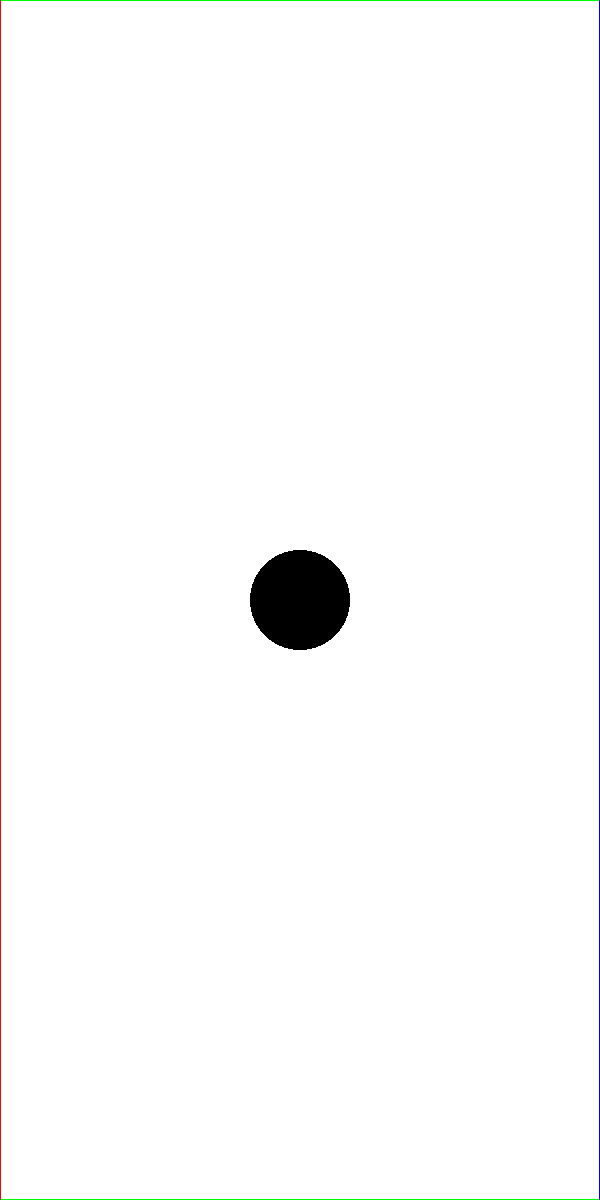
\includegraphics[width=.5\linewidth]{../prob1HR.png}
  \captionof{figure}{The set up for problem 1}
  \label{fig:test1}
\end{minipage}%
\begin{minipage}{.5\textwidth}
  \centering
  \includegraphics[width=.6\linewidth]{../prob24.png}
  \captionof{figure}{The set up for the edge coupled stripline}
  \label{fig:test2}
\end{minipage}
\end{figure}



\section{Methods 1: Solving Numerically For a General Case}
 The numerical solver functions, called in the main program, solve for a grid of points that is filled with user defined boundary conditions. To create the grid a user creates an image with colours corresponding to voltages, grounds and other boundary conditions (see Figure 1). Figures 2, 3 and 4 are examples of such input images. The image is processed by a grid function such that it can be solved for using the numerical methods that follow. A solution grid of potential is returned. \\
(TODO: REFER TO PESUDOCODE OR ACTUAL CODE FILE grid.cpp) \\ 
\\
A separate function calculates the E-field grid, i.e the gradient of the potential field, according to~(\ref{eq:efield}) using a symmetric derivative method. The difference in values across the adjacent cells per unit cell are used as an approximation for the derivative for each cell. The derivative is calculated in this way for all points except outer points using a for loop.\\
(TODO: HOW ARE OUTER POINTS DEALT WITH)
\\
(TODO: REFER TO PESUDOCODE OR ACTUAL CODE GradientGrid.cpp) \\
 \\
\\



\subsection{The Finite Difference Method}
The first of the numerical methods implemented was the finite difference method. We need to solve Laplace's equation~(\ref{eq:laplace}) for a specified grid. First write in terms of a cartesian coordinate system:  
\begin{equation}
\frac{\partial^2\phi}{\partial x^2}+\frac{\partial^2\phi}{\partial y^2}=0
\label{eq:lapcart}
\end{equation}  
If we substitute the above derivatives in \textit{x} and \textit{y} using centre difference expressions, i.e
\begin{multicols}{2}
  \begin{equation}
\frac{\partial^2\phi}{\partial x^2} = \frac{\phi_{x+1,y}-2\phi_{x,y}+\phi_{x-1, y}}{h^2}
  \end{equation}\break
  \begin{equation}
\frac{\partial^2\phi}{\partial y^2} = \frac{\phi_{x,y+1}-2\phi_{x,y}+\phi_{x, y-1}}{h^2}
  \end{equation}
\end{multicols}
 n.b \textit{h} = \Delta\)\textit{x} = \Delta\textit{y}\) since our grid is symmetric.\\
\\
we can then rearrange to arrive at an expression for potential at some point in terms of adjacent points:
\begin{equation}
\phi_(x,y) = \frac{1}{4}(\phi_{x+1,y}+\phi_{x-1,y}+\phi_{x,y+1} + \phi_{x, y-1})
\label{eq:fdm}
\end{equation}
\\
provided boundary conditions are provided. \\
 \\
This method is implemented in the program by looping over all of the points in the input grid that provides such boundary conditions and thus creating a new solution grid for potential according to~(\ref{eq:fdm}). 

\subsection{Improving The Finite Difference Method: \textit{SOR}}
-involves using our current result at each point~(\ref{eq:laplace}) as an intermediate stage \\
-and then calculating the actual new value according to \\
\begin{equation}
\phi_{x,y}^{New} = (1-\omega)\phi_{x,y}+\omega\phi_{x,y}^{Intermediate}
\label{eq:sor}
\end{equation}



\subsection{Matrix Inversion Method}
-the maths \\
-how it is implemented in program \\

\subsection{A Third Method?} \\
-maths \\
-implementation \\



\section{Methods 2: Analysing Results}
-general structure of analysis section of program (how results are analysed) \\
-quantifying error in each numerical method \\
-comparing to analytical solutions \\
-comparing between numerical methods \\
-presentation of  results, comparisons and error \\

\section{Methods 3: The User Interface ??}
-how we added to the program in order to make it efficient and easy to use \\
-how the user interface works \\


\section{Results and Discussion}
-numerical results for all three problems\\
-metadata for runs \\
-comparison between numerical and analytical results where applicable\\
-comparison between different methods of numerical solvers\\

\section{Conclusion and Outlook}
-evaluation of the project - what went well - what would be improved if repeated (not just in terms of quality of results but also CPU cost\\
-might be nice for chris to explain how he has already optimised things compared to previous versions of the program \\
-outlook for further work e.g extending the software etc \\

\newpage
\section{Appendix 1 - Analytical Solutions}
In order to solve for our situation (Figure 2) that demonstrates circular symmetry Laplace's equation is first converted to polar form:
\begin{equation}
\vec{\nabla}^2\phi = \frac{\partial^2\phi}{\partial r^2}+\frac{1}{r}\frac{\partial\phi}{\partial r}+\frac{1}{r^2} \frac{\partial^2\phi}{\partial\theta^2}=0
\label{6}
\end{equation}
As there is no \theta\) dependence for this situation the term containing the second derivative of \phi\) with respect to \theta\) disappears and the differential equation, no longer partial, becomes:
\begin{equation}
\vec{\nabla}^2\phi = \frac{\partial^2\phi}{\partial r^2}+\frac{1}{r}\frac{\partial\phi}{\partial r}=0
\label{8}
\end{equation}
and is now easily solvable by first introducing a function to reduce order:


\begin{equation}
\lambda(r) = \frac{\partial\phi}{\partial r}
\label{10}
\end{equation}
to rewrite the differential equation as follows: 
\begin{equation}
\lambda ' + \frac{1}{r}\lambda = 0.
\label{11}
\end{equation}
This is trivial to solve for \lambda\) and thus first derivative of potential,  i.e:
\begin{equation}
\lambda(r) =  \frac{\partial\phi}{\partial r} = ke^{-\ln|r|} = \frac{k}{r}
\label{11}
\end{equation}
where \textit{k} is some constant.
\begin{equation}
 \frac{\partial\phi}{\partial r} = \frac{k}{r}
\label{11}
\end{equation}
The first order differential equation (11) is now trivial to separate and solve and we arrive at a general solution for potential:
\begin{equation}
\phi = k\ln|r| + C
\label{11}
\end{equation}
Using the fact that potential is 0 at R_i\) and V at R_o\) as boundary conditions gives the particular form of potential as (6). \\
\includepdf{A1.pdf}
\includepdf{A2.pdf}
\includepdf{A22.pdf}
\includepdf{A31.pdf}
\includepdf{A32.pdf}
\includepdf{CM1.pdf}
\includepdf{CM2.pdf}








\end{document}
